%
% loesung.tex -- Beispiel-File für die Beschreibung der Loesung
%
% (c) 2020 Prof Dr Andreas Müller, Hochschule Rapperswil
%
\section{Lösung
\label{legendre:section:loesung}}
\rhead{Lösung}
\subsection{Bedeutung $l$- und $m$-Richtung
\label{legendre:subsection:lmrichtung}}
Wie schon im vorherigen Abschnitt (\ref{legendre:section:problemstellung}) angesprochen, gibt es zwei Parameter, $l$ für den Grad und $m$ für die Ordnung.
Mit den Bedingungen für die beiden Parameter ($l\geq 0$ und $m=0, \ldots , l$) ergibt sich eine bestimmte Struktur von möglichen zugeordneten Legendrepolynomen.
Diese Struktur ist in Abbildung \ref{legendre:fig:struktur} dargestellt.
% Plot Legendrepolynome Struktur
\begin{figure}[!h]
\centering
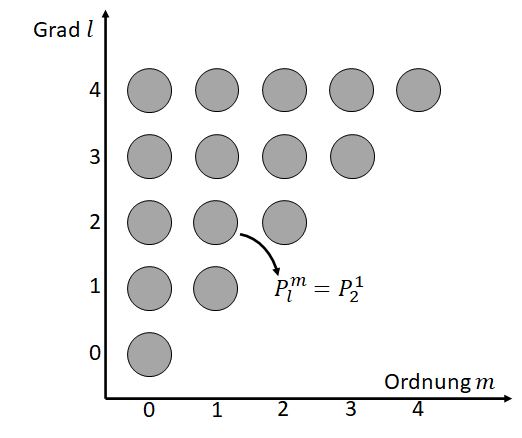
\includegraphics[width=0.6\linewidth]{papers/legendre/plots/legendre_struktur}
\caption{Ausschnitt aus der Struktur der möglichen zugeordneten Legendrepolynome.}
\label{legendre:fig:struktur}
\end{figure}
Die beiden Gleichungen \eqref{legendre:recurrence-l} und \eqref{legendre:recurrence-m} aus dem vorherigen Abschnitt (\ref{legendre:section:problemstellung}) unterscheiden sich in der Rekursionsrichtung.
Während die Rekursion mittels Gleichung \eqref{legendre:recurrence-l} in $l$-Richtung verläuft, sprich in Richtung des Grades, verläuft die Rekursion mittels Gleichung \eqref{legendre:recurrence-m} in $m$-Richtung, sprich in Richtung der Ordnung.

\subsection{Anfangswerte
\label{legendre:subsection:anfangswerte}}
Jede Rekursionsbeziehung braucht seine Anfangswerte.
So werden auch für die beiden Rekursionsformeln \eqref{legendre:recurrence-l} und \eqref{legendre:recurrence-m} je zwei Anfangswerte benötigt.
Für die Rekursionsformel in $l$-Richtung \eqref{legendre:recurrence-l} werden die Anfangswerte $P^{l}_{l}$ \eqref{legendre:pll} und $P^{l}_{l+1}$ \eqref{legendre:pllp1} benötigt.
Für die Rekursionsformel in $m$-Richtung \eqref{legendre:recurrence-m} wird mittels $P^{l}_{l}$ aus der Gleichung \eqref{legendre:pll} die beiden Anfangswerte $P^{l}_{l+1}$ \eqref{legendre:pllp1} und $P^{l+1}_{l+1}$ \eqref{legendre:plp1lp1} berechnet.
Bei der Gleichung \eqref{legendre:pll} für den Anfangswert $P^{l}_{l}$ gilt es zu beachten, dass $!!$ für die Doppelfakultät steht und nicht für die Fakultät der Fakultät.
% Anfangswert P^{l}_{l}
\begin{equation}
P^{l}_{l}(x)
=(-1)(2l-1)!!(1-x^2)^{l/2}
\label{legendre:pll}
\end{equation}
% Anfangswert P^{l}_{l+1}
\begin{equation}
P^{l}_{l+1}(x)
=x(2l+1)P^{l}_{l}(x)
\label{legendre:pllp1}
\end{equation}
% Anfangswert P^{l+1}_{l+1}
\begin{equation}
P^{l+1}_{l+1}(x)
=-(2l+1)\sqrt{1-x^2}P^{l}_{l}(x)
\label{legendre:plp1lp1}
\end{equation}
In der Einleitung (\ref{legendre:section:einleitung} wurde bereits erwähnt, dass die Rekursionsformeln weniger Rechenaufwand benötigen als die direkte Formel \eqref{legendre:geschlosseneform}.
Dies gilt auch noch unter Einbezug dieser Anfangswerte.

\subsection{Rekursionsformel in $m$-Richtung
\label{legendre:subsection:mrichtung}}
Für die Abbildung \ref{legendre:fig:plot-m} wurde das zugeordnete Legendrepolynom mit Grad 50 und Ordnung 3 mittels der Rekursionsbeziehung \eqref{legendre:recurrence-m} in $m$-Richtung berechnet.
Die Anfangswerte $P^{l}_{l+1}$ \eqref{legendre:pllp1} und $P^{l+1}_{l+1}$ \eqref{legendre:plp1lp1} geben vor, dass bei Verwendung dieser Rekursionsbeziehung diese in negativer $m$-Richtung verläuft.
Dazu muss die Rekursionsgleichung \eqref{legendre:recurrence-m} etwas umgeformt werden.
Daraus entsteht die neue Rekurstionsgleichung in $m$-Richtung \eqref{legendre:recurrence-m-neu}.
% umgeformte Rekursionsformel in m-Richtung
\begin{equation}
P^{m-1}_{l}(x)
= \left[ \frac{2mxP^{m}_{l}(x)}{- \sqrt{1-x^2}}-P^{m+1}_{l} \right]
\frac{1}{(l+m)(l-m+1)}
\label{legendre:recurrence-m-neu}
\end{equation}
Wird die umgeformte Rekursionsgleichung \eqref{legendre:recurrence-m-neu} auf numerische Instabilität untersucht, fällt sofort der Term $\sqrt{1-x^2}$ auf.
Dieser Term deutet darauf hin, dass nahe an den Intervallsgrenzen ($x \rightarrow \pm 1$) Auslöschung auftreten kann.
Dies alleine ist noch nicht allzu schlimm.
Jedoch ist es so, dass die zugeordneten Legendrepolynome für $m>0$ an den Intervallsgrenzen Null ergeben.
Das heisst, dass die Differenz in der eckigen Klammer nahe den Intervallsgrenzen in etwa Null ergibt.
Der Term $\sqrt{1-x^2}$, welcher von Auslöschung betroffen ist, wird nahen den Intervallsgrenzen sehr klein und bläst somit den Term $2mxP^{m}_{l}(x)$ auf, welcher dadurch selbst fehlerhaft wird.
Die Differenz in der eckigen Klammer unterliegt somit einer quasi-Auslöschung.
In der eckigen Klammer werden zwei fast gleich grosse Terme voneinander Subtrahiert, wobei der erste Term durch die Auslöschung und das Aufblasen durch $\sqrt{1-x^2}$ selbst stark fehleranfällig ist.

Es stellt sich nun die Frage, warum diese numerische Instabilität nicht im Graphen \ref{legendre:fig:plot-m} ersichtlich ist, wie beispielsweise in dem Graphen \ref{legendre:fig:wolframalpha} den Wolfram Alpha erstellt.
Eine Antwort darauf liefert der Term $\frac{1}{(l+m)(l-m+1)}$, welcher einen positiven Einfluss bezüglich numerischer Fehler hat.
Dadurch, dass die Rekursionsgleichung zwei Anfangswerte hat, ist $l\geq m+2$ gegeben.
Damit lässt sich der Nenner dieses Terms auf $\geq 6$ abschätzen, was wiederum bedeutet, dass $\frac{1}{(l+m)(l-m+1)} \leq \frac{1}{6}$ ist.
Dadurch verkleinert sich der Wert der Differenz in der eckigen Klammer der Rekursionsgleichung und ein Teil des Fehlers wird somit eliminiert.
Sprich, einige fehlerhafte stellen hinter dem Komma verschwinden.
Diese Rekursionsgleichung bleibt jedoch fehleranfällig nahe den Intervallsgrenzen, falls numerische Fehler aus einer anderen Quelle einfliessen, wie beispielsweise fehlhafte oder ungenaue Anfangswerte.

\subsection{Rekursionsformel in $l$-Richtung
\label{legendre:subsection:lrichtung}}
Für die Abbildung \ref{legendre:fig:plot-l} wurde ebenfalls das zugeordnete Legendrepolynom mit Grad 50 und Ordnung 3 berechnet, jedoch mit der Rekursionbeziehung \eqref{legendre:recurrence-l} in $l$-Richtung.
Die Anfangswerte $P^{l}_{l}$ \eqref{legendre:pll} und $P^{l}_{l+1}$ \eqref{legendre:pllp1} zeigen, dass die Rekursion in positiver $l$-Richtung verläuft.
Daher muss bei der Gleichung \eqref{legendre:recurrence-l} nur noch der Faktor $(l-m+1)$ auf die rechte Seite gebracht werden.
Dies führt zur neuen Rekursionsformel in $l$-Richtung \eqref{legendre:recurrence-l-neu}.
% umgeformte Rekursionsformel in l-Richtung
\begin{equation}
P^{m}_{l+1}(x)
= \frac{(2l+1)xP^{m}_{l}(x)-(l+m)P^{m}_{l-1}(x)}{(l-m+1)} 
\label{legendre:recurrence-l-neu}
\end{equation}
Bei einem Vergleich mit der Rekursionsformel in $m$-Richtung (siehe Gleichung \eqref{legendre:recurrence-m-neu} fällt auf, dass der Term $\sqrt{1-x^2}$ in dieser Rekursionsgleichung nicht vorhanden ist.
Auch sonst ist kein Term vorhanden, der nahe den Intervallsgrenzen eine numerische Instabilität hervorrufen könnte.
Jedoch gilt es noch die Faktoren vor den Legendrepolynomen zu untersuchen.
Diese beiden Faktoren sind $\frac{(2l+1)}{(l-m+1)}$ und $\frac{(l+1)}{(l-m+1)}$.
Gegeben durch die Anfangswerte ist mit dem gleichen Argument wie im vorherigen Abschnitt \ref{legendre:subsection:mrichtung} wieder gegeben, dass $l\geq m+2$ ist.
Daraus lässt sich ableiten, dass $\frac{(2l+1)}{(l-m+1)}\geq 1$ für $m>0$ ist und dass $\frac{5}{3}\leq \frac{(l+1)}{(l-m+1)}<2$.
Da die beiden Faktoren jeweils $\geq 1$ sind, bedeutet dies, dass die Fehler in den Polynomen $P^{m}_{l}$ und $P^{m}_{l-1}$ vergrössert werden.
Daraus lässt sich schliessen, dass diese Rekursionsbeziehung fehleranfällig ist, falls numerische Fehler aus einer anderen Quelle einfliessen, wie beispielsweise fehlerhafte oder ungenaue Anfangswerte.

\subsection{Welche Rekursionsformel soll nun verwendet werden?
\label{legendre:subsection:welche}}
Es stellt sich die Frage, welche der beiden Rekursionsformeln verwendet werden soll?
Die in $l$-Richtung \eqref{legendre:recurrence-l-neu}? Oder doch die in $m$-Richtung \eqref{legendre:recurrence-m-neu}?
Denn obwohl die beiden Graphen (vergleiche Abbildung \ref{legendre:fig:plot-l} mit \ref{legendre:fig:plot-m}) optisch gleich aussehen, gibt es Unterschiede.
Der Graph in Abbildung \ref{legendre:fig:plot-diff} zeigt die Differenz der beiden Graphen aus Abbildung \ref{legendre:fig:plot-l} und Abbildung \ref{legendre:fig:plot-m}.
Es ist deutlich zu sehen, dass sich die beiden Rekursionsformeln nahe den Intervallsgrenzen unterscheiden.
Die Analyse der Rekursionsbeziehung in $m$-Richtung aus Abschnitt \ref{legendre:subsection:mrichtung} lässt vermuten, dass diese dafür verantwortlich ist.
Dies spricht dafür, die Rekursionsbeziehung in $l$-Richtung zu verwenden.
Ein weiterer Punkt, der für die Rekursionsbeziehung in $l$-Richtung spricht, ist, dass die GNU Scientific Library \cite{legendre:gsl} diese Implementation mit den gleichen Anfangswerten wie in Abschnitt \ref{legendre:subsection:anfangswerte} verwendet.
Die Implementation der GNU Scientific Library wird allgemein als numerisch stabil angesehen.
% Plot in l-Richtung
\begin{figure}[!h]
\centering
\includegraphics[width=1.0\linewidth]{papers/legendre/plots/plot_diff_l_m}
\caption{Differenz zweier zugeordneten Legendrepolynome mit Grad 50 und Ordnung 3, einmal berechnet mit der Rekursionsformel in \texorpdfstring{$l$}{l}-Richtung und einmal berechnet mit der Rekursionsformel in \texorpdfstring{$m$}{m}-Richtung.}
\label{legendre:fig:plot-diff}
\end{figure}
